\documentclass[12pt]{article}
\usepackage{color,graphicx}
\usepackage{hyperref}
\textwidth 170mm
\textheight 210mm
\topmargin 0.0mm
\oddsidemargin 0mm
\evensidemargin 0mm
\parindent 0pt

\begin{document}
\pagenumbering{arabic}

\vspace{10 mm}
\Huge
ANT.UI: User Manual\vspace{10 mm}
\normalsize

\begin{abstract}
ANT.UI is a graphical interface designed to streamline the construction of molecular junction inputs for ANT.Gaussian (ANT). The application allows users to build a complete junction geometry from scratch in real time, manipulating electrodes and molecules interactively in three dimensions, and to export ready-to-run input files for ANT and Gaussian with a single click. Advanced sequential-output tools further extend these capabilities, enabling automated electrode-pulling sequences, surface scans, and step-wise rotation studies. Together, these features substantially reduce the time required to set up transport calculations, both for experienced ANT users and for newcomers to theoretical molecular electronics.
\end{abstract}

\section{Installation and configuration}

ANT.UI is a Python application and can be run directly from its source files. Python~3.8 or later is required, along with the packages listed in \texttt{requirements.txt}. Install them with:

\begin{verbatim}
pip install -r requirements.txt
\end{verbatim}

On Linux, \texttt{tkinter} is not bundled with the default Python installation and must be installed separately via the system package manager (e.g.\ \texttt{sudo apt install python3-tk} on Debian/Ubuntu). On Windows and macOS it is included with the standard Python installer.

To launch the application, run:

\begin{verbatim}
python ANT.UI.py
\end{verbatim}

Alternatively, a standalone executable can be compiled with PyInstaller using the command at the top of \texttt{ANT.UI.py}.

\subsection*{Configuration file}

Before using ANT.UI for the first time, edit the \texttt{USER\_CONF.txt} file to match your cluster environment. The file is parsed by searching for the delimiter \texttt{\#\%\%}, reading the keyword on the following line, and treating all subsequent lines up to the next \texttt{\#\%\%} as the value for that keyword. Any text outside a keyword block is ignored, so the file can be freely annotated or used to store multiple cluster configurations.

The supported keywords are:

\begin{itemize}
    \item \textbf{ANTDIRcall}: Path to the ANT installation directory on the cluster, containing the modified \texttt{L502} and \texttt{L101} Gaussian link files. All new users must set this.

    \item \textbf{JOBHEAD}: Header lines written at the top of the generated \texttt{launchANT.sh} submission script. Tailor this to your cluster's scheduler (e.g.\ PBS or Slurm) and set the number of cores here.

    \item \textbf{GAUSSIANHEAD}: Opening lines of the Gaussian input file (memory, processor count, etc.). The number of processors should match the value set in \textbf{JOBHEAD}.

    \item \textbf{G09call}: The command used to invoke Gaussian on your cluster (e.g.\ \texttt{g09}). If your cluster calls Gaussian with a different command, set it here.

    \item \textbf{PYTHONcall}: The command used to invoke Python~3 on the cluster (e.g.\ \texttt{python3}). ANT.UI embeds Python helper scripts in sequential outputs that are launched via this call.

    \item \textbf{ANTpredet}: Fixed lines written to the \texttt{.ant} input file for every job. These correspond to the standard ANT convergence and accuracy parameters. Additional keywords may be appended automatically by ANT.UI depending on the calculation type.

    \item \textbf{ZMAX}: Upper limit in Ångström of the z-position slider for the top electrode. Defaults to $20.0$~Å. Increase this value if your junction geometry requires a larger electrode separation.

    \item \textbf{U\_ELECTRON\_SCREENING}: Multiplicative factor applied to the DFT+U Hubbard parameter before it is written to the \texttt{.ant} file. Defaults to $1.0$. A value of $0.7$ is typical and accounts for the screening of the bare molecular $U$ by the metallic electrodes. See Section~\ref{sec:dftu} for details.
\end{itemize}

\newpage
\section{The user interface}

The purpose of ANT.UI is to construct the three-dimensional geometry of a molecular junction interactively. The junction consists of three components — a bottom electrode, a molecule, and a top electrode — whose relative positions fully define the input geometry. ANT.UI allows the user to move the top electrode and the molecule independently; the bottom electrode acts as the fixed reference frame.

\begin{figure}[h]
    \centering
    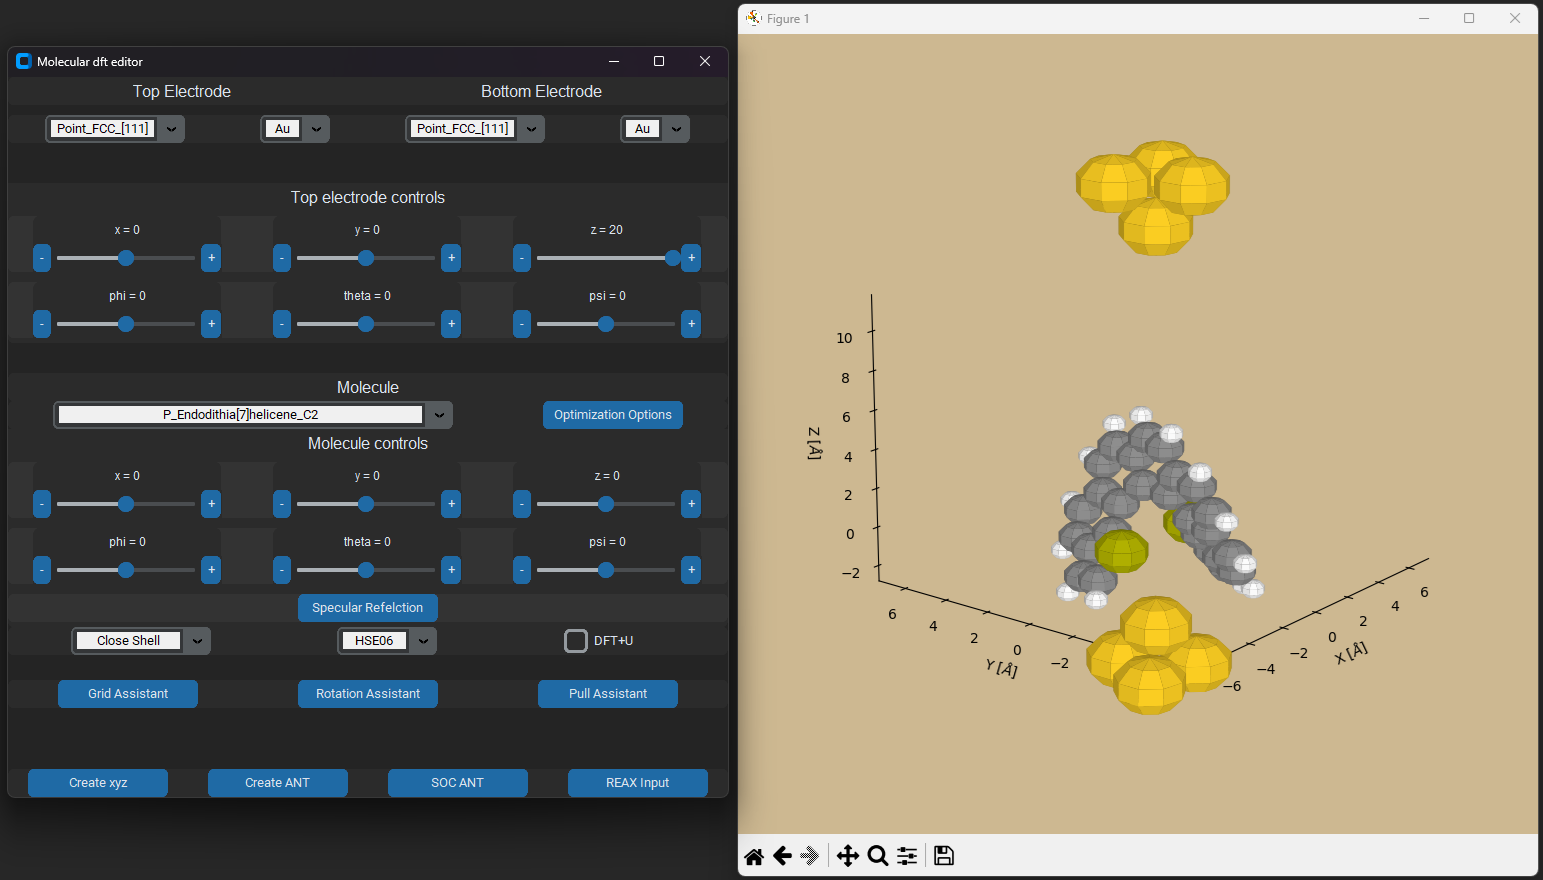
\includegraphics[width=1\linewidth]{Figures/Fig1.png}
    \caption{The ANT.UI interface, showing the controller window (left) and the 3D viewer (right).}
    \label{fig:UI}
\end{figure}

As shown in Fig.~\ref{fig:UI}, the interface consists of two windows: the \textbf{controller} and the \textbf{viewer}. The viewer renders an interactive 3D representation of the junction. The outermost two layers of each electrode are hidden in the viewer because they serve as Bethe-lattice anchor layers in ANT and are treated differently from the rest of the structure. The controller provides all controls for modifying the geometry, selecting components, and configuring DFT settings.

The controller is organised from top to bottom as follows.

\subsubsection*{Electrode configuration}

The first row allows the user to select the electrode type and element independently for the top and bottom electrodes. Electrode geometries are stored as XYZ files in the \texttt{ElectrodesDFT} folder; users may add custom geometries to this folder at any time. All electrode files in the folder must use gold atoms as a template, since other elements are obtained by rescaling the gold geometry with the appropriate lattice-parameter ratio. All files must represent a \emph{top} electrode; ANT.UI applies a rotation automatically when the same geometry is assigned as the bottom electrode.

\subsubsection*{Top electrode controls}

The next section contains the position and orientation controls for the top electrode. The upper row of sliders translates the electrode along the $x$, $y$, and $z$ axes; the lower row rotates it around each axis. Note that ANT requires the Bethe lattice to be aligned along the $z$ axis, so rotating the electrode about the $x$ or $y$ axis is generally not recommended.

\subsubsection*{Molecule selection}

A pre-loaded catalogue of molecules is available from the \textbf{Molecule} drop-down menu. To add a custom molecule, place an XYZ-format text file in the \texttt{Molecules} subfolder; the new entry will appear in the menu after restarting the application. The XYZ format expected by ANT.UI is:

\begin{verbatim}
12
LSDA 3.5 | PBE 4.0
C  0.000  0.000  0.000
H  1.000  0.000  0.000
...
\end{verbatim}

The first line is the atom count. The second line is the comment line and may optionally contain DFT+U values for one or more functionals (see Section~\ref{sec:dftu}); leave it blank if DFT+U is not needed. Each subsequent line gives an element symbol followed by $x$, $y$, $z$ coordinates in Ångström. To generate a purely metallic junction without a molecule, select the \texttt{PureMetallic} entry.

The \textbf{Optimization Options} button, located on the same row as the molecule selector, opens the optimization configuration window described in Section~\ref{sec:opt}.

\subsubsection*{Molecule controls}

The molecule controller mirrors the top-electrode controller. An additional \textbf{Specular Reflection} button is provided for chiral molecules: pressing it applies a mirror reflection to all atomic coordinates, toggling the handedness of the molecule without requiring a second file.

\subsubsection*{DFT settings}

This row sets the electronic-structure parameters for the output files: the spin treatment (closed shell or open shell), the exchange-correlation functional (chosen from a list of common options), and optionally DFT+U (see Section~\ref{sec:dftu}). The \textbf{Abs.\ Energy} checkbox, when enabled, instructs ANT.UI to include an additional Python script in the output that records the absolute DFT energy at each step of a sequential calculation. This is useful for constructing potential-energy curves alongside transport data, for example during an electrode-pulling sequence.

\subsubsection*{Advanced functionalities}

The three buttons in this row — \textbf{Pull Assistant}, \textbf{Grid Assistant}, and \textbf{Rotation Assistant} — open pop-up windows for generating sequential outputs. These are described in detail in Section~\ref{sec:adv}. Read that section before using them.

\subsubsection*{Output creation}

The final row contains the output buttons. Pressing any of them creates a new subfolder inside the \texttt{Outputs} directory; the folder name is derived from the molecule name and an index to ensure uniqueness.

\begin{itemize}
    \item \textbf{Create xyz}: writes only the XYZ coordinate file for the junction geometry.
    \item \textbf{Create ANT}: generates all input files required to run a transport calculation with ANT (Gaussian \texttt{.gjf}, ANT \texttt{.ant}, and a submission script \texttt{launchANT.sh}).
    \item \textbf{SOC ANT}: generates the same set of files as \textbf{Create ANT} but with spin-orbit coupling enabled, provided the electrode element is supported (see Section~\ref{sec:soc}).
\end{itemize}

\section{General workflow}

The recommended procedure for building a junction and generating outputs is as follows.

\begin{itemize}
    \item \textbf{Select all components first.} Choose the electrode type and element for both electrodes, and select the molecule, \emph{before} making any positional adjustments. Changing the electrode element after moving it does not reset its position, but it does rescale the geometry, which will shift atoms from their intended locations.

    \item \textbf{Position the molecule, then the top electrode.} The bottom electrode is fixed and serves as the reference. It is easiest to first bring the molecule into contact with the bottom electrode using the molecule sliders, and then lower the top electrode to complete the junction.

    \item \textbf{Configure DFT settings.} The functional, spin treatment, and optimization options are persistent across the session; they can be set at any point and will apply to all subsequent outputs.

    \item \textbf{Generate outputs.} Once the geometry and settings are finalised, press the appropriate output button. Multiple outputs can be generated in a single session; creating an output does not alter any positional or DFT settings.
\end{itemize}

\section{Basis sets}

ANT.UI assigns basis sets to atoms depending on their role in the junction.

\textbf{Bethe-lattice support atoms} (the two outermost layers of each electrode) are assigned a minimal basis. ANT.UI looks for a file named \texttt{Element\_CRENBS.gbs} (e.g.\ \texttt{Au\_CRENBS.gbs}) in the \texttt{DFT\_min\_basis\_pseudopot} folder. Each file must follow the Gaussian format: the basis set first, then the pseudopotential, separated by \texttt{****}.

\textbf{Standard electrode atoms} (the layers shown in the viewer) are assigned a larger basis. ANT.UI looks for a matching file in \texttt{DFT\_basis\_pseudopot} using the same naming convention. If no file is found for a given element, \texttt{lanl2dz} is used as the default.

\textbf{Molecule atoms} always use \texttt{lanl2dz}.

Custom basis sets can be added to either folder at any time; the files are loaded at startup.

\section{Spin-orbit coupling}\label{sec:soc}

ANT supports spin-orbit coupling (SOC) calculations through a specialised set of basis functions and SOC parameters. The files required for this are stored in the \texttt{SOC\_params} folder. Only elements with entries in this folder support the \textbf{SOC ANT} output button; if either electrode element is unsupported, the button is disabled automatically. The currently supported elements are: Au, Pt, Cu, Ag, Al, and Ni.

\section{Optimization}\label{sec:opt}

Geometry optimisation of the junction can be performed in Gaussian before the transport calculation. The \textbf{Optimization Options} window, opened from the main controller, configures how the structure is relaxed.

\begin{figure}[h]
    \centering
    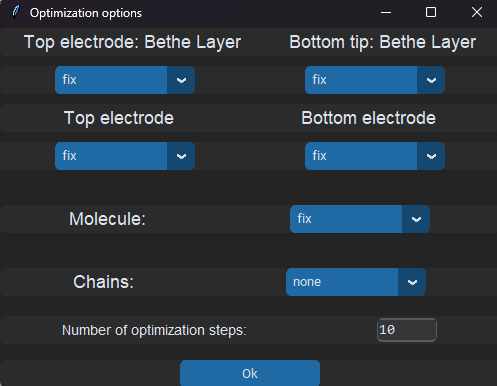
\includegraphics[width=0.5\linewidth]{Figures/Fig2.png}
    \caption{The Optimization Options window.}
    \label{fig:opt}
\end{figure}

As shown in Fig.~\ref{fig:opt}, the window is divided into five regions corresponding to the five structural components: the Bethe-lattice support layer and the active region of each electrode, and the molecule. Each region can be assigned one of the following optimisation modes:

\begin{itemize}
    \item \textbf{fix} — atoms in this region are frozen.
    \item \textbf{z} — atoms are allowed to relax only along the $z$ axis.
    \item \textbf{all} — atoms are free to relax in all three directions.
\end{itemize}

The Bethe-lattice support layers are restricted to \textbf{fix} or \textbf{z} only, since the lattice structure of these layers must be preserved for ANT to attach the semi-infinite electrodes correctly. When \textbf{z} is chosen for a support layer, all atoms in a given layer move as a rigid block, preserving the planar geometry.

The molecule has an additional option, \textbf{all, some z}, which opens a sub-window where the indices of specific atoms can be entered. Those atoms will be constrained to move only along $z$, while the rest of the molecule remains free. This is useful for preventing the molecule from drifting laterally during optimisation.

The \textbf{Chains} option controls how optimisation interacts with the advanced sequential outputs:

\begin{itemize}
    \item \textbf{none} — no optimisation is performed at any step.
    \item \textbf{first step} — only the first geometry in the sequence is optimised in Gaussian; all subsequent geometries are generated from the relaxed first-step structure.
    \item \textbf{every step} — each step in the sequence is initialised from the optimised output of the previous one, forming a chain of relaxations. This is the most computationally intensive option but produces the most physically realistic sequence.
\end{itemize}

The \textbf{Number of optimization steps} field sets the maximum number of optimisation cycles passed to Gaussian. Molecular junctions are challenging systems for standard geometry optimisers and rarely reach the default convergence thresholds. A value between 10 and 30 steps is usually sufficient for most practical junctions.

When any optimisation mode is active, ANT.UI includes a Python connector script in the output folder. This script reads the Gaussian output and constructs the ANT input from the relaxed geometry. To disable ANT in the pipeline and run only the Gaussian optimisation, remove the \texttt{L502} and \texttt{L101} substitution lines from both the connector script and the Gaussian input file.

\newpage

\section{DFT+U}\label{sec:dftu}

DFT+U is an ANT feature that corrects the Kohn-Sham gap of a molecule by adding a Hubbard-$U$ parameter to the GGA Hamiltonian. The appropriate value of $U$ can be estimated from isolated-molecule Gaussian calculations using:

\begin{equation}
    U_{\mathrm{GGA}} = \left|E_{\mathrm{HOMO}}^{\mathrm{KS}} - \bigl(E[n+1] - E[n]\bigr)\right| + \left|E_{\mathrm{LUMO}}^{\mathrm{KS}} - \bigl(E[n] - E[n-1]\bigr)\right|
\end{equation}

where $E[n]$ is the total DFT energy of the molecule with $n$ electrons ($n$ being the number of electrons of the neutral species), and $E_{\mathrm{HOMO}}^{\mathrm{KS}}$ and $E_{\mathrm{LUMO}}^{\mathrm{KS}}$ are the frontier orbital energies from the Kohn-Sham calculation.

Once $U$ has been computed for a given molecule and functional, store it in the comment line (second line) of the molecule's XYZ file. For example, to assign $U = 2.86$~eV for the PBE functional, write \texttt{PBE 2.86} on that line. Multiple functionals can be listed simultaneously, separated by \texttt{|}:

\begin{verbatim}
PBE 2.86 | BLYP 2.52
\end{verbatim}

The DFT+U checkbox in the main controller becomes active only when the selected molecule has a stored $U$ value for the currently chosen functional. When checked, ANT.UI writes the necessary ANT keywords to the \texttt{.ant} file. The value written is scaled by the \textbf{U\_ELECTRON\_SCREENING} factor from \texttt{USER\_CONF.txt} (default $1.0$; a value of $0.7$ is commonly used to account for metallic screening of the molecular $U$).

\newpage
\section{Advanced functionalities}\label{sec:adv}

The three advanced-functionality buttons open pop-up windows for creating \emph{sequential outputs}: sets of related ANT inputs that together constitute a multi-step calculation. The relationship between steps depends on the chosen assistant and the optimisation chain setting from Section~\ref{sec:opt}. Pressing \textbf{Ok} in any of these windows generates the full output sequence in the \texttt{Outputs} folder.

    \subsection{Pull Assistant}

    The Pull Assistant generates a sequence of outputs in which the electrode separation is varied in uniform steps along the $z$ axis, simulating the stretching or compression of a junction.

    \begin{figure}[h]
        \centering
        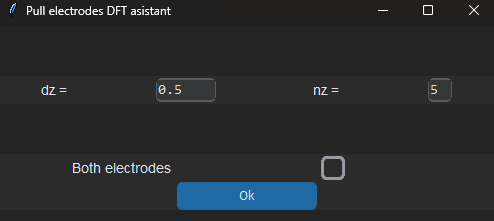
\includegraphics[width=0.5\linewidth]{Figures/Fig3.png}
        \caption{The Pull Assistant window.}
        \label{fig:pull}
    \end{figure}

    The user specifies the total number of steps $n_z$ and the per-step displacement $dz$ (in Ångström). If \textbf{Both electrodes} is unchecked, only the top electrode moves by $dz$ per step. If it is checked, each electrode moves by $dz/2$ in opposite directions, so the total gap changes by $dz$ per step. A positive $dz$ corresponds to stretching (pulling); a negative $dz$ corresponds to compression (pushing).

    Each step produces a complete set of ANT input files. When optimisation is enabled, the necessary Python connector scripts and a master submission script are also generated. Note that the master script provides a convenient starting point but may require adaptation to your specific cluster configuration.

    The Pull Assistant combined with \textbf{every step} optimisation produces a sequence that closely approximates a quasi-static break-junction simulation.

    \subsection{Grid Assistant}

    The Grid Assistant generates a two-dimensional grid of outputs by scanning the top electrode over a set of lateral positions at fixed height. This mimics an STM measurement where the transmission is evaluated at each grid point.

    \begin{figure}[h]
        \centering
        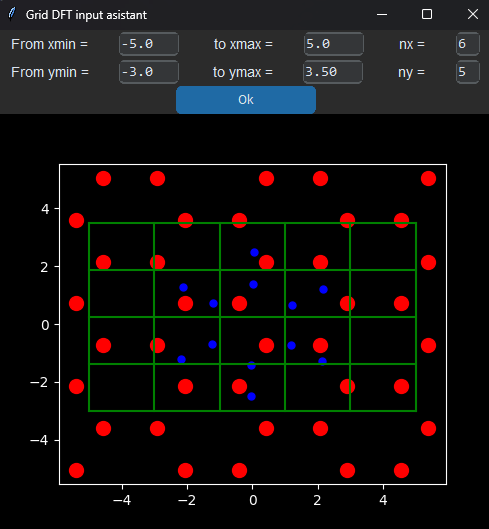
\includegraphics[width=0.5\linewidth]{Figures/Fig4.png}
        \caption{The Grid Assistant window, shown here with a benzene molecule on a gold slab.}
        \label{fig:scan}
    \end{figure}

    The pop-up displays a top-down view of the junction: molecule atoms in blue, bottom-electrode atoms in red, and the user-defined grid in green. The user sets the $x$ and $y$ limits of the scan area and the number of grid points in each direction. The height of the top electrode ($z$ coordinate) is taken from the current session state and held constant across the scan; only the lateral position of the tip varies.

    Combining the Grid Assistant with \textbf{first step} optimisation is a practical strategy: the molecule is first relaxed in place, and the grid scan then uses the relaxed geometry as its starting point.

    \subsection{Rotation Assistant}

    The Rotation Assistant generates a sequence of outputs in which a selected part of the junction is rotated about the $z$ axis by a uniform angular increment. This is useful for studying how conductance varies with the relative orientation of a molecule or electrode.

    \begin{figure}[h]
        \centering
        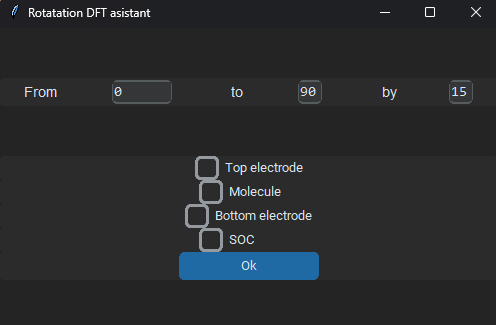
\includegraphics[width=0.5\linewidth]{Figures/Fig5.png}
        \caption{The Rotation Assistant window.}
        \label{fig:twist}
    \end{figure}

    The user selects which component to rotate (top electrode, molecule, or bottom electrode), the starting and ending angles (in degrees), and the number of angular steps. The \textbf{SOC} checkbox generates the sequence with spin-orbit coupling enabled.

    Before committing to a full rotation sequence, it is advisable to use the manual rotation sliders in the main controller to preview a few intermediate orientations and verify that the resulting geometries are physically reasonable.

\newpage
    \subsection{Examples of use}

    Figure~\ref{fig:Example} illustrates several applications of the advanced-output tools using benzene and C$_{60}$ fullerene as test molecules.

    \begin{figure}[h]
        \centering
        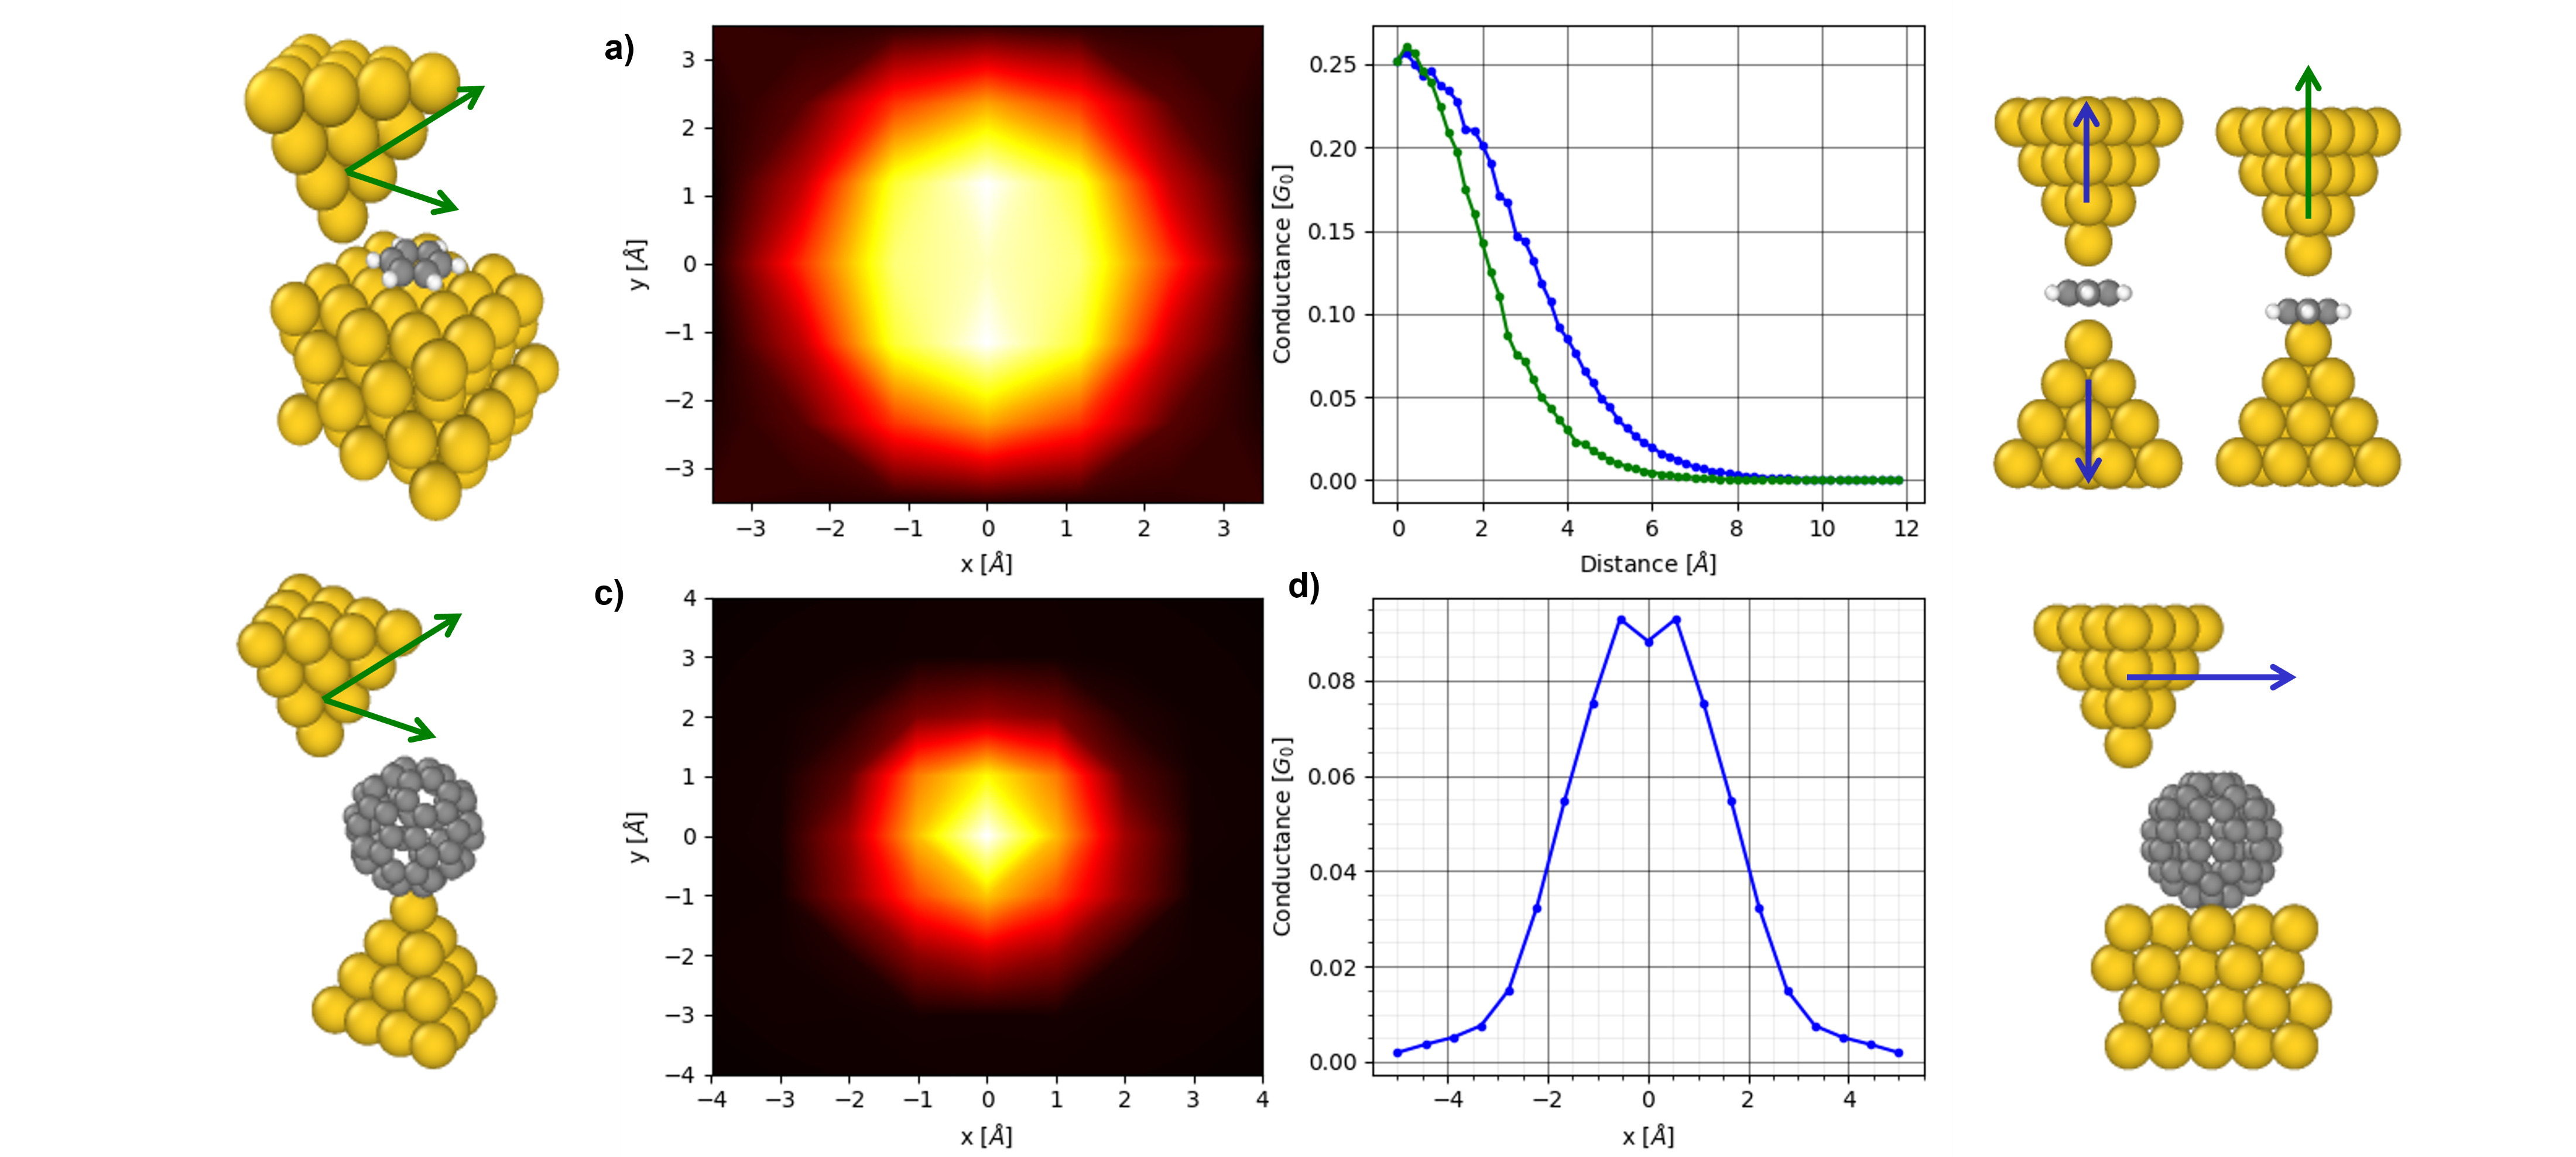
\includegraphics[width=1\linewidth]{Figures/Fig6.png}
        \caption{Examples of advanced-functionality outputs. (a)~Transmission contour map from a grid scan of benzene on a gold slab. (b)~Transmission as a function of electrode separation from a pull sequence on benzene, comparing the case where both electrodes move symmetrically (blue) with the case where only the top electrode moves (green). (c)~Grid scan of a C$_{60}$ fullerene on a gold tip. (d)~Single-line scan over a fullerene on a slab, showing the transmission profile along the scan direction.}
        \label{fig:Example}
    \end{figure}


\section{Multiple molecules in one input}

ANT treats all non-metallic atoms in the input as a single ``molecule'', regardless of whether they form one connected fragment or several. This behaviour can be exploited to simulate transport through multi-molecule junctions.

ANT.UI does not provide a dedicated tool for this scenario, but the following manual procedure works reliably. Set up the electrodes and place the first molecule in its desired position, then generate an output. Without moving the electrodes, reposition the molecule to the second desired location and generate a second output. Repeat for each molecule. Finally, open the Gaussian input files from all outputs and copy the atomic coordinates of each molecule into a single input file. When doing so, the atom indices used to identify the top-electrode region in the ANT input must be updated to account for the extra atoms that have been inserted.

Alternatively, a multi-molecule arrangement can be saved as a single XYZ file in the \texttt{Molecules} folder. ANT.UI will treat it as one object, and the geometry optimisation tools can then be used to refine the arrangement in the usual way.

\end{document}
